
\chapter{序論}
\label{chap:introduction}

本章ではWeb上におけるテキスト表示についての現状、Web上での書き手側の文章(日本語テキスト)の特色を述べ、
それを踏まえて本論⽂の目的、ならびに構成について述べる。

\newpage

\section{研究動機}

コンピューター技術の発展、およびスマートフォンやタブレット端末(モバイル端末)の普及に伴い、
人は読む文章を映し出されたものへと推移しつつある。また、ブログやSNSといったウェブサービスの台頭が加わり、
ウェブ上に文章や画像といったコンテンツを共有し、それを閲読、ないしリアクションをもらう機会に恵まれるようになった。
\\一方で、多種多様なデバイスが普及されたことにより、ブラウザやアプリケーションのデザインは表示形式は
その画面サイズに依存した表示(レスポンシブ)となる。よってその書き手側の表示環境と読み手側の表示環境は異なる場合がある。
以下の画像はAndroid,iPhone,PCブラウザ上でTwitterのタイムラインを表示した場合の画面である。
画面のサイズに依存して横幅が異なることで文章のレイアウト自体が変化するしていることが分かる。

\begin{figure}[H]
    \centering
    \label{fig:image1}
    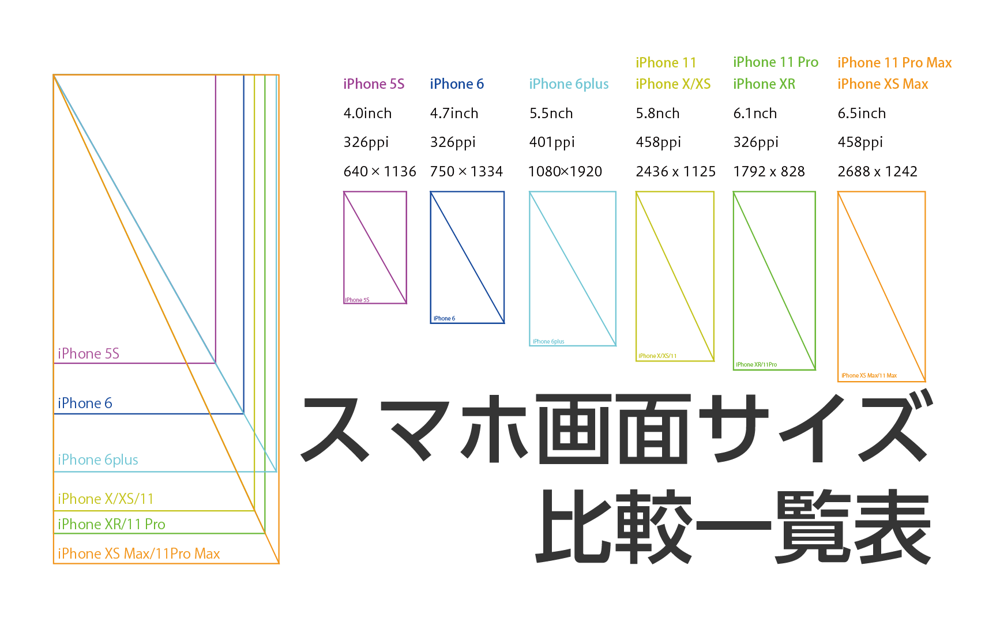
\includegraphics[width=0.7\columnwidth]{image/01/img1.png}
    \caption[スマホの画面の比較] {スマホの画面の比較\footnotemark[1]}
\end{figure}

\footnotetext[1]{
    引用元 \protect\url{
        https://developer.android.com/training/multiscreen/screensizes?hl=ja.
    }
}

\begin{figure}[H]
    \begin{tabular}{cc}
        \begin{minipage}[t]{0.5\hsize}
            \centering
            \label{fig:image2}
            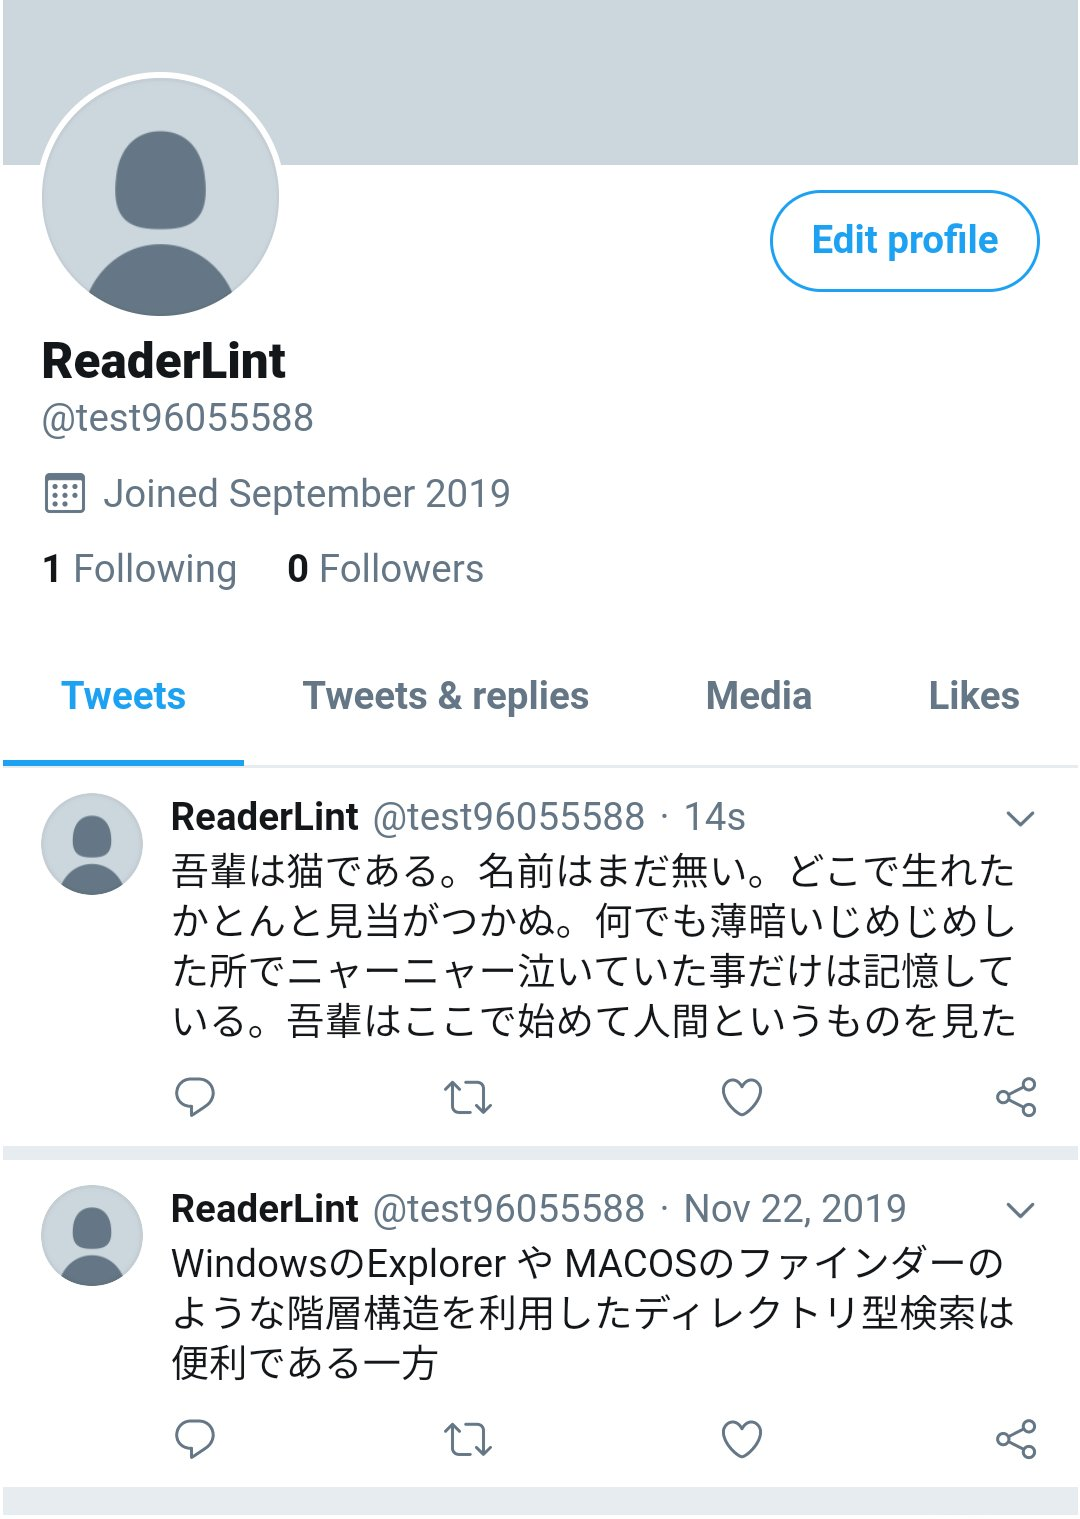
\includegraphics[keepaspectratio, width=0.5\columnwidth]{image/01/img3.jpg}
            \caption[Androidにおける] {スマホの画面の比較}
        \end{minipage}&

        \begin{minipage}[t]{0.5\hsize}
            \centering
            \label{fig:image3}
            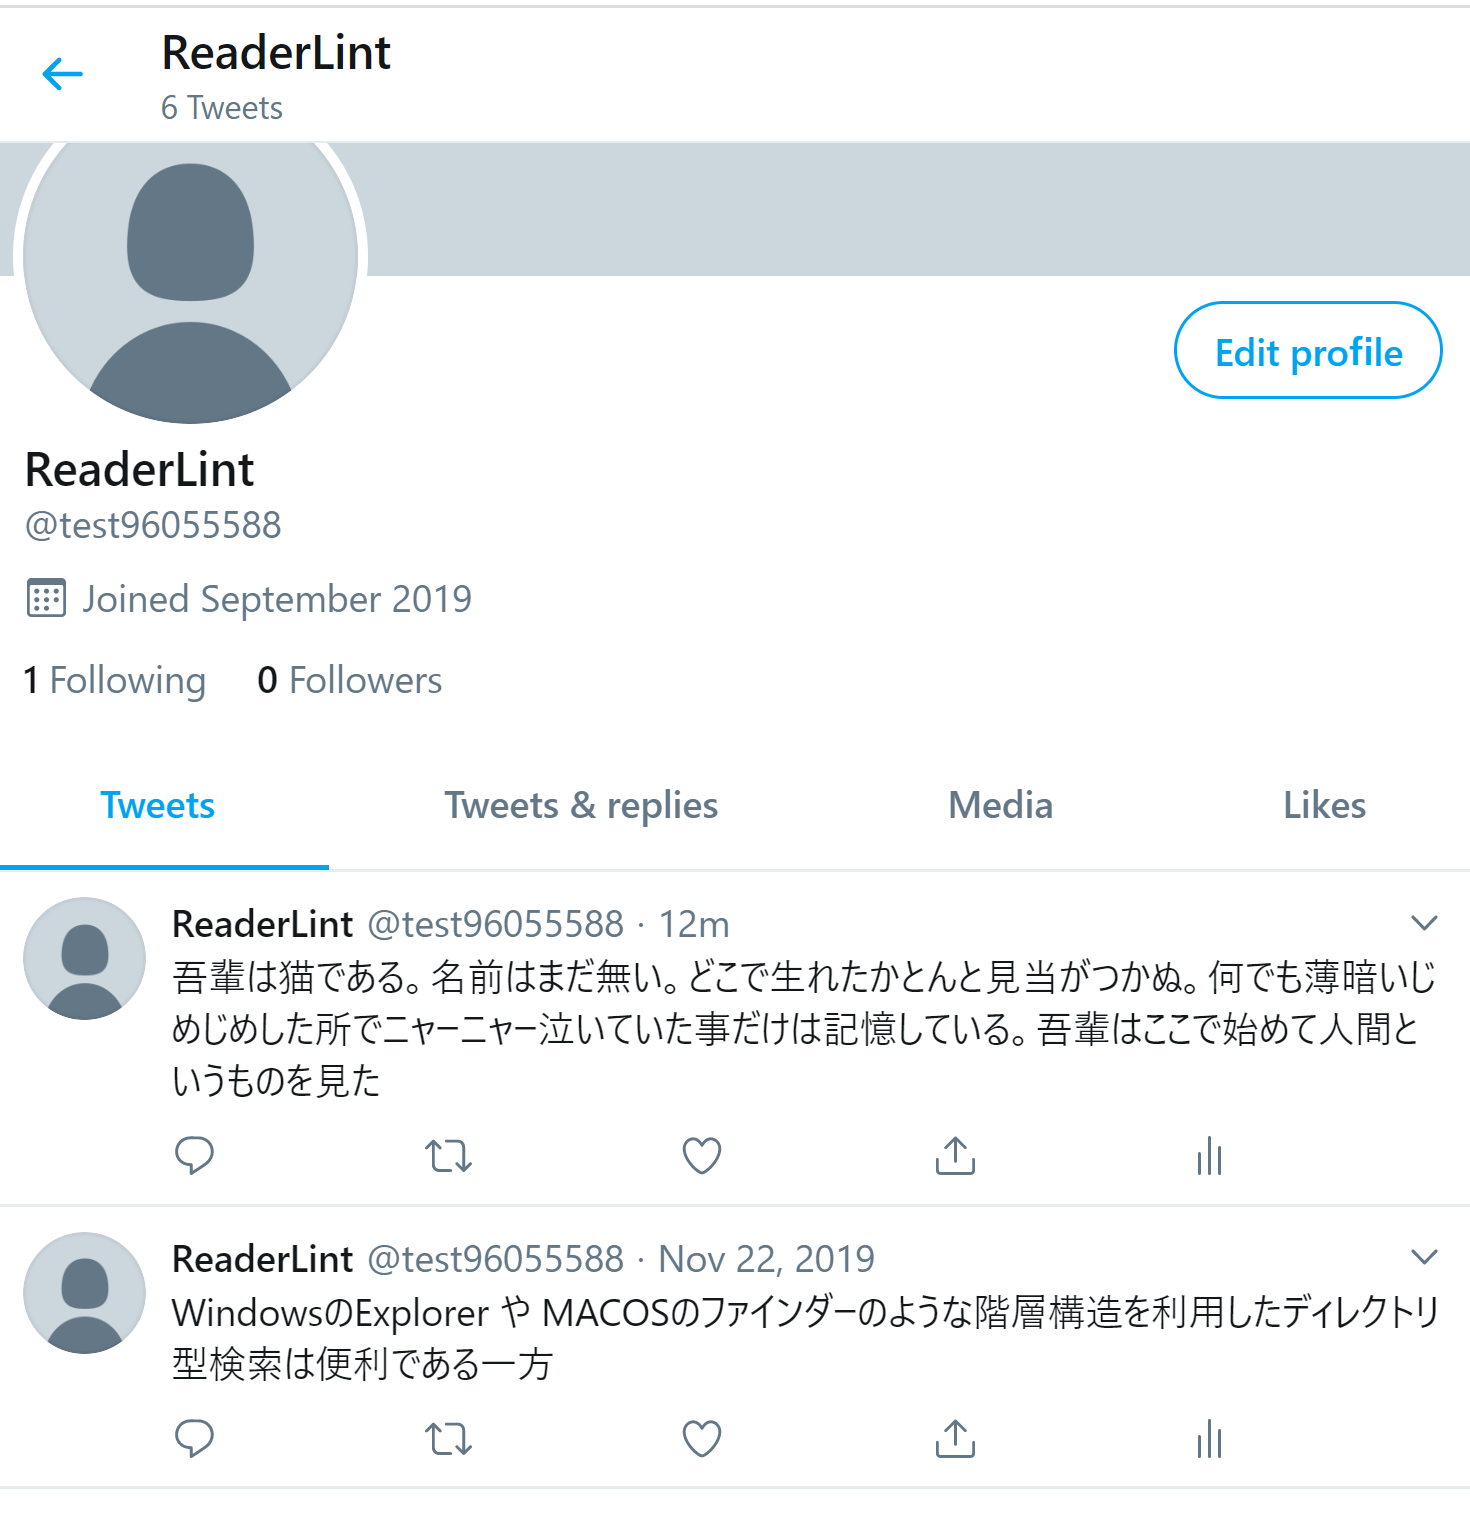
\includegraphics[keepaspectratio, width=0.5\columnwidth]{image/01/img4.png}
            \caption[PCブラウザにおける] {PCブラウザにおける}
        \end{minipage}
    \end{tabular}
\end{figure}

また、同じデバイスを用いても多様なクライアントを想定するアプリケーションにおいて、
そのクライアントアプリのデザインの仕様によって異なる表示になる。
\\このとき、各デバイスのテキストエリアのサイズに従って打たれたテキストは、
別環境で表示されたときに崩れたレイアウトになることで、
可読性を損ねる場合があり、読み手側のストレスとなりえるケースが発生する。
\\このようなケースは書き手側が自身のWYSIWYGエディタや表示環境での
視認性を高めるため、意図的に改行を入れているため発生するため、
文章のレイアウトの型崩れはブラウザで修正することは困難であった。

つづいて文章レイアウトの問題として日本語の改行問題を取り上げる。
日本語の改行問題の詳細は『Budou:日本語のための自動折り返し制御ツール』\footnotemark[4]の
紹介ページから引用する。
\begin{quotation}
    ウェブページ上の日本語の文章は、行末に置かれると、単語の途中でも折り返されてしまうことがあります。
    皆さんも、以下のような文章を見たことがあるはずです。「新しい Android の世界へようこそ。」という見出しの
    「ようこそ」という単語が、「ようこ」と「そ」の間で折り返され、ひとまとまりの単語として認識しにくくなっています。
    このように、単語の途中で発生する折り返しは、文章の読みやすさを下げる一因です。
    \begin{figure}[H]
        \centering
        \label{fig:image4}
        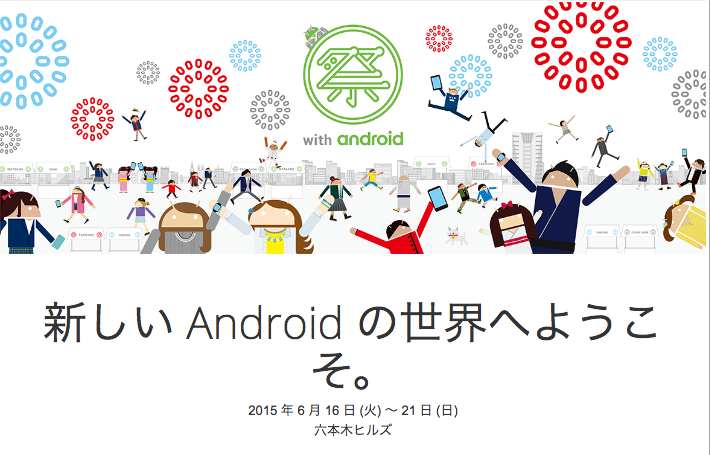
\includegraphics[width=0.7\columnwidth]{image/01/img2.png}
        \caption[単語の途中で折り返しが発生している例] {単語の途中で折り返しが発生している例}
    \end{figure}
\end{quotation}

このようにWeb上の日本語の文章のレイアウトに関しては独自の問題がある。また、上記の画像では文末の字余りが例として出されていたが、
以下の画像における一行目の文末に「どこで」のいち「ど」が一文字だけが表示されるパターン、
4行目の文頭で「ニャーニャー」のうち「ャー」だけが表示されるパターンも、ひとまとまりの文意として認識しづらくなっている。
    \begin{figure}[H]
        \centering
        \label{fig:image5}
        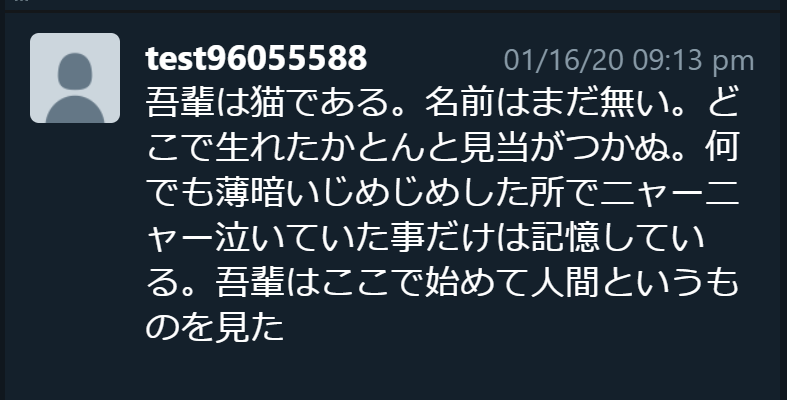
\includegraphics[width=0.7\columnwidth]{image/01/img5.png}
        \caption[ひとまとまりの文意を損ねている例] {ひとまとまりの文意を損ねている例}
    \end{figure}

\section{本研究の目的}
本研究では書き手と読み手のデバイスの違いや、表示形式の違いに生まれる文章構成の誤差によって生まれる
文章レイアウトの崩れを解消し、読み手側に対してより可読性の高い文章を表示するようにフォーマットすることで
ユーザビリティを損ねなさせない表示を提供するシステムの開発を目的とする。

\section{本論文の構成}
 本論⽂は本章を含めた6章で構成される。
 \\第2章では、本研究に関連した研究、およびライブラリを紹介した上で問題点を整理する。
 \\第3章では、本論⽂で提案するシステムの基本構成と使い⽅について述べる。
 \\第4章では、ユーザーからのフィードバックをまとめ、本論⽂で提案する
システムの有効性と問題点について述べる。
 \\最後に、第5章で本論⽂のまとめと結論を述べる。
